% Based on Model 1 from "Activity 5 - Binary" by Helen Hu
% which in turn uses "Count the Dots" from csunplugged.org

\model{Binary Numbers}

Each team has four cards that are ordered from the card with the most dots (8) to the card with the least dots (1).
The cards represent four binary digits, or in other words, a 4-bit number.

\newcommand{\bin}[4]{#1\hspace{64pt}#2\hspace{64pt}#3\hspace{64pt}#4}

\begin{center}
\begin{tabular}{|c|C{1in}|}
\hline
Binary & Decimal \\
\hline

\includegraphics[height=1in]{CSP/binary1.png} & \\
\bin{1}{0}{1}{0} & \ans{10} \\
\hline

\includegraphics[height=1in]{CSP/binary2.png} & \\
\bin{1}{0}{1}{1} & \ans{11} \\
\hline

\includegraphics[height=1in]{CSP/binary3.png} & \\
\bin{1}{1}{0}{0} & \ans{12} \\
\hline
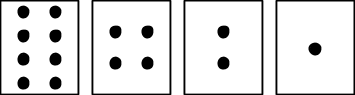
\includegraphics[height=1in]{CSP/binary4.png} & \\
\bin{1}{1}{1}{1} & \ans{15} \\
\hline
\end{tabular}
\end{center}


\quest{15 min}


\Q \label{fourbit} In the table above, write the decimal value for each row by counting the number of dots.
\begin{enumerate}
\item What is the largest decimal number that can be represented by four bits? \ans{15}
\item What is the smallest decimal number that can be represented by four bits? \ans{0}
\item How many possible decimal numbers can be represented by four bits? \ans{16}
\end{enumerate}


\Q Examine the binary notation below the cards.
Explain in a full sentence what a 0 means about the card's dots and what a 1 means.

\begin{answer}
0 means the card is turned over and the dots don't count, and 1 means the dots count in that binary number.
\end{answer}


\Q \label{binhex} Complete the following table by writing the binary representation of the decimal numbers 0 to 15 using four bits.
(And check your answers for \ref{fourbit}.)

\begin{center}
\begin{tabular}{|C{1in}|C{1in}|C{1in}|}
\hline
Decimal & Binary & Hex \\
\hline
0  & \ans{0000} & 0 \\
\hline
1  & \ans{0001} & 1 \\
\hline
2  & \ans{0010} & 2 \\
\hline
3  & \ans{0011} & 3 \\
\hline
4  & \ans{0100} & 4 \\
\hline
5  & \ans{0101} & 5 \\
\hline
6  & \ans{0110} & 6 \\
\hline
7  & \ans{0111} & 7 \\
\hline
8  & \ans{1000} & 8 \\
\hline
9  & \ans{1001} & 9 \\
\hline
10 & \ans{1010} & A \\
\hline
11 & \ans{1011} & B \\
\hline
12 & \ans{1100} & C \\
\hline
13 & \ans{1101} & D \\
\hline
14 & \ans{1110} & E \\
\hline
15 & \ans{1111} & F \\
\hline
\end{tabular}
\end{center}


\Q \emph{Hexadecimal} is shorthand for binary. For example, 0xD5 in hex is 1101 0101.

\begin{enumerate}
\item What is 0x2E in binary? \ans{0010 1110}
\item What is 0x74 in binary? \ans{0111 0100}
\item What is 0xB00 in binary? \ans{1011 0000 0000}
\item What is 0xFAD in binary? \ans{1111 1010 1101}
\end{enumerate}


\Q Based on the table in \ref{binhex}, explain why binary is sometimes referred to as base-2, decimal as base-10, and hexadecimal as base-16.

\begin{answer}
In base-2, there are two possible digits: 0 and 1.
In base-10, there are ten possible digits: 0--9.
In base-16, there are sixteen possible digits: 0--9 and A--F.
\end{answer}


\Q Explain the humor: ``There are only 10 types of people in the world: those who understand binary, and those who don't.''

\begin{answer}
The number 10 in binary is 2 in decimal.
So there are only two types of people in the world.
\end{answer}


\Q Typically computers group 8 bits together at a time (8 bits are also called 1 \emph{byte}).
Fill in the number of dots for the four new cards: \ans{128 ~ 64 ~ 32 ~ 16}

\begin{center}
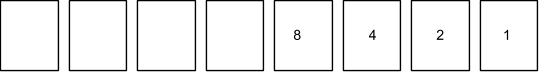
\includegraphics[width=\textwidth]{CSP/binary5.png}
\end{center}


\Q What is the largest number that can be represented by:
\begin{enumerate}
\item five bits? \ans{31}
\item six bits? \ans{63}
\item seven bits? \ans{127}
\item eight bits? \ans{255}
\item $n$ bits? \ans{$2^n - 1$}
\end{enumerate}


\Q Most computers built since the year 2000 have 64-bit processors.
Before then, 32-bit processors were the norm.
What is the advantage of having more bits?

\begin{answer}
All data on a computer (text, images, sounds) are represented with numbers.
With more bits, the processor can represent larger values and thus support more complex information.
\end{answer}


\Q In terms of logic gates and digital circuits, what is the disadvantage of having more bits?

\begin{answer}
Since bits are implemented with logic gates, they take up physical space.
The more bits, the larger the processor (and other hardware) needs to be and the more power it will consume.
\end{answer}
